 \documentclass{beamer}

\usepackage{ucs}
\usepackage[utf8x]{inputenc}
\usepackage[T1]{fontenc}
\usepackage[english]{babel}
\usepackage[retainorgcmds]{IEEEtrantools}%	IEEEeqnarray
\usepackage{mathabx}%	convolution symbol
\usepackage{multi row}
\usepackage{listings}

\usepackage{epstopdf}

\usepackage{subfig}
\usepackage{algpseudocode}
\usepackage{algorithmicx}
\usepackage{algorithm}
\usepackage{relsize}%	relative font sizes
\usepackage{multicol}
\usepackage{multirow}
\usepackage{todonotes}
\usepackage{xspace}

\lstset{
	language=C++,
	basicstyle=\footnotesize,
	showtabs=true,
	tabsize=3,
}

%	presentation info
\title{Optimization of a Finite-Volume Method Application}

\author{José Alves, Rui Brito}

\institute[22765, 22781]{
	Universidade do Minho
}

\date{Braga, June 2013}


%	beamer options
\usetheme{CambridgeUS}


\begin{document}%	begin presentation

\maketitle%	title slide

\begin{frame}
	\frametitle{Index}
	\tableofcontents
\end{frame}

\section{Introduction}
\begin{frame}
	\frametitle{conv-diff (Recap)}
	\begin{description}
		\item [What?] Computes the heat diffusion of a fluid spreading over an area;
		\item [How?] Uses a Finite-Volume method;
		\item [Why?] Represents surface as a mesh, making each cell only dependent of its neighbours;
	\end{description}
\end{frame}

\begin{frame}
	\begin{figure}[!htp]
    	\centering   
        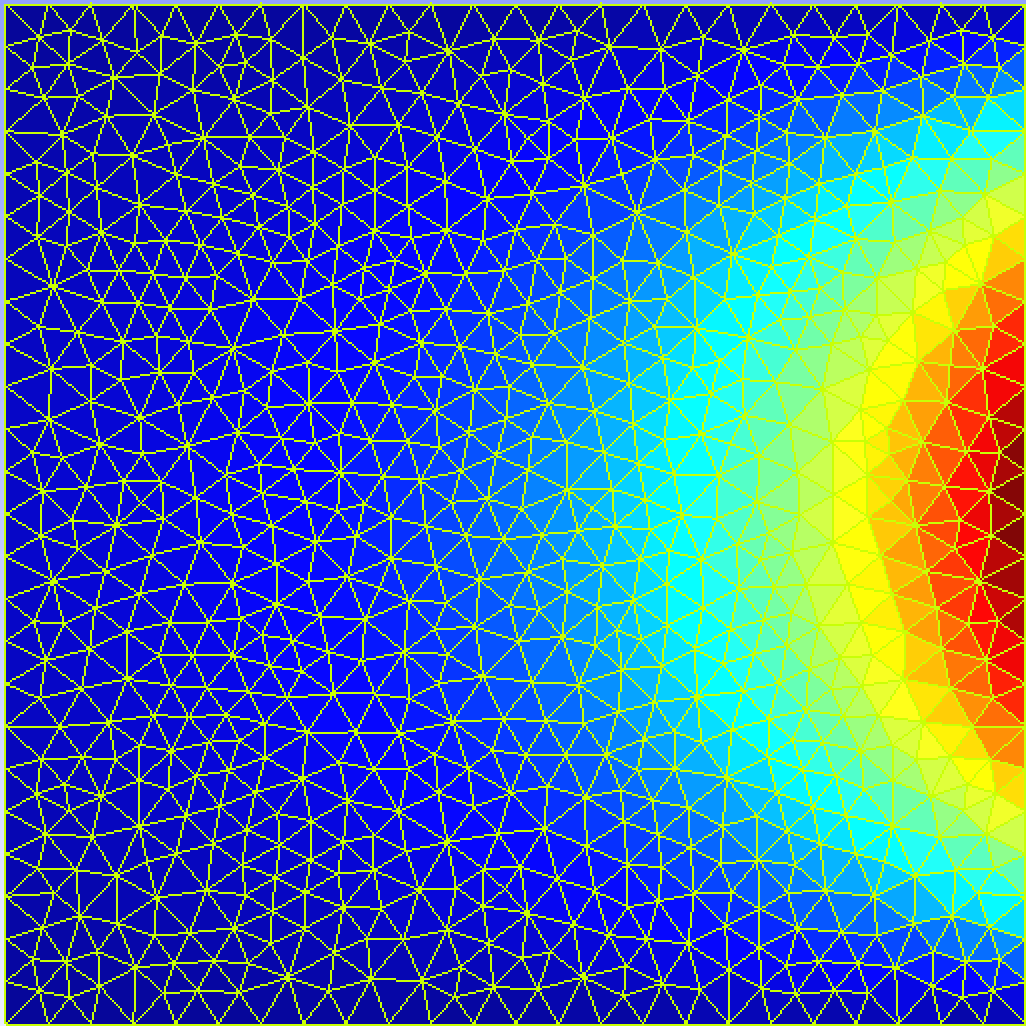
\includegraphics[width=.6\textwidth]{../images/mesh.png}        
	\end{figure}
\end{frame}

\begin{frame}
	The main objective is to compute a vector $\overline{\phi}$ such that $\overline{\phi} \longrightarrow G(\overline{\phi}) = \left(\begin{array}{c}
	0\\ 
	0\\
	\vdots\end{array}\right)$
	This is accomplished in three different stages:
	\begin{enumerate}
	    \item {We begin with a candidate vector $\phi$} 
	    \item {For each edge, we compute the flux $F_{ij}$, with $i$ and $j$ being the indexes of the adjacent cells}
	    \item {For each cell, we compute $\sum |e_{ij}| F_{ij} - |c_i| f_i$}
	\end{enumerate}
	Thus: $\phi = \left(\begin{array}{c}
	\phi_1\\
	\vdots\\
	\phi_I
	\end{array}\right) \longrightarrow G = \left(\begin{array}{c}
	G_1\\
	\vdots\\
	G_I
	\end{array}\right)$
\end{frame}

\begin{frame}
	\begin{description}
		\item [makeFlux] Compute the contribution from each edge;
		\item [makeResidual] Compute the $\phi$ vector, adding the flux for each cell from each contribution;	
	\end{description}
\end{frame}

\section{Original Implementation}

\begin{frame}
	\frametitle{Original implementation}
	\begin{itemize}
		\item \textbf{\itshape Arrays-of-Pointers};				
	\end{itemize}

	\begin{columns}
		\column{.45\textwidth}		
		\begin{block}{makeFlux}
			
			For all \textbf{edges}:
			\begin{enumerate}
				\item Read adjacent cell data;	
				\item Compute edge velocity;
				\item Compute flux through edge;				
			\end{enumerate}
		\end{block}

		\column{.45\textwidth}		
		\begin{block}{makeResidual}
			
			For all \textbf{edges}:
			\begin{enumerate}
				\item Subtract flux from right cell;
				\item Add flux to left cell;
			\end{enumerate}
		\end{block}
	\end{columns}
\end{frame}

\section{Tests}

\begin{frame}[plain]
	\frametitle{Test Machines (for most of the project)}
		\begin{center}

			\begin{table}[!htp]
			\resizebox{\textwidth}{!}{
			\begin{tabular}{|c|c|c|c|c|}
			\hline
			 & compute-511@search & compute-601@search & compute-101@search & MacBookPro\\
			 & AMD Opt 6174 & Xeon X5650 & Xeon E7520 & Intel Ivy-Bridge i7\\
			\hline
			\# processors & 2 & 2 & 2 & 1\\
			\# cores per processor & 12 & 6 & 1 & 4\\
			hyper-threading & - & yes & yes & yes\\
			clock frequency(GHz) & 2.2 & 2.66 & 3.2 & 2.3\\
			L1 capacity & 128KB & 32KB & 16KB & 64KB\\
			L2 capacity & 512KB & 256KB & 2MB & 256KB\\
			L3 capacity & 12MB & 12MB & - &6MB\\
			RAM capacity & 64GB & 48GB & 2GB & 16GB\\
			\hline
			\end{tabular}}
			\caption{Test machines}			
			\end{table}
		\end{center}
\end{frame}


\section{Optimizations}

\subsection{Naive Optimizations}

\begin{frame}
	\frametitle{Naive Optimizations}	
		\begin{itemize}
		\item Removed redundant loads and calculations;
		\item Changed some variable definitions to \emph{const};
		\item Usage of a recent compiler auto-optimizations(SLP);				
	\end{itemize} 	
\end{frame}

\subsection{OpenMP}

\begin{frame}
	\frametitle{Identified Problems}
	\begin{itemize}
	\item High number of memory accesses;
	\item Low operational intensity;
	\item Deep memory indirection chain;
	\item Bad data locality;
	\end{itemize}
\end{frame}

\begin{frame}	
	\begin{center}

	\begin{figure}[!htp]
		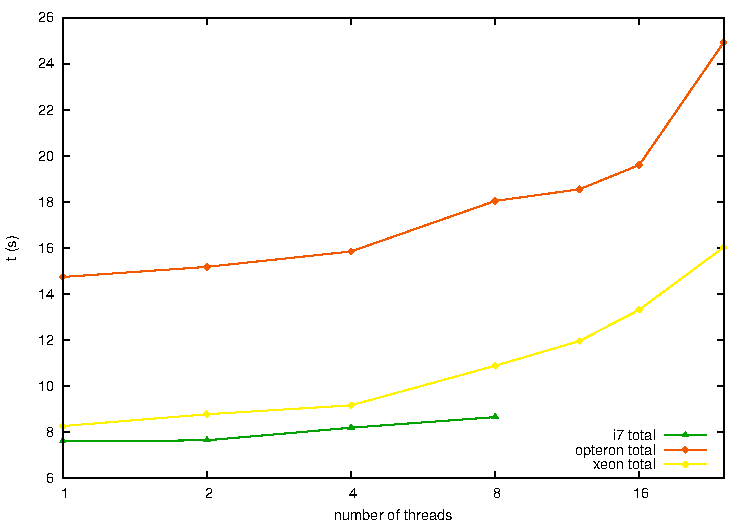
\includegraphics[width=9cm]{../images/total.pdf}
		\caption{Total application runtime}
		\label{fig:roofline}
	\end{figure}
	\end{center}
\end{frame}

\begin{frame}
	\begin{center}
	\begin{figure}[!htp]
		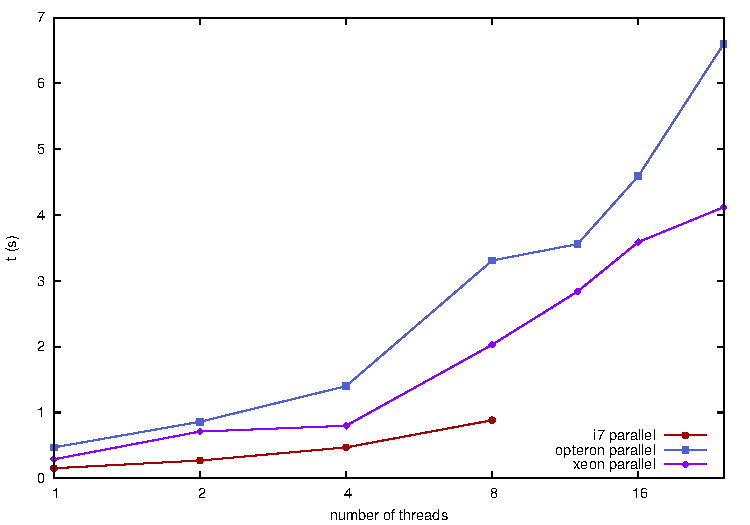
\includegraphics[width=9cm]{../images/parallel.pdf}
		\caption{Parallel section runtime}
		\label{fig:roofline}
	\end{figure}
	\end{center}
\end{frame}

\subsection{MPI} 

\begin{frame}
	\frametitle{Problems}
	\begin{itemize}		
		\item High level of communication between processes;
		\item High level of barrier synchronization;
		\item Some balancing problems;
		\item Computed error spikes;
		\item Some of FVLib's templates are hard to serialize (locality);
		\item Sequential portion is slow;
	\end{itemize}		
\end{frame}



\begin{frame}
	\begin{figure}[!htp]
    	\centering   
        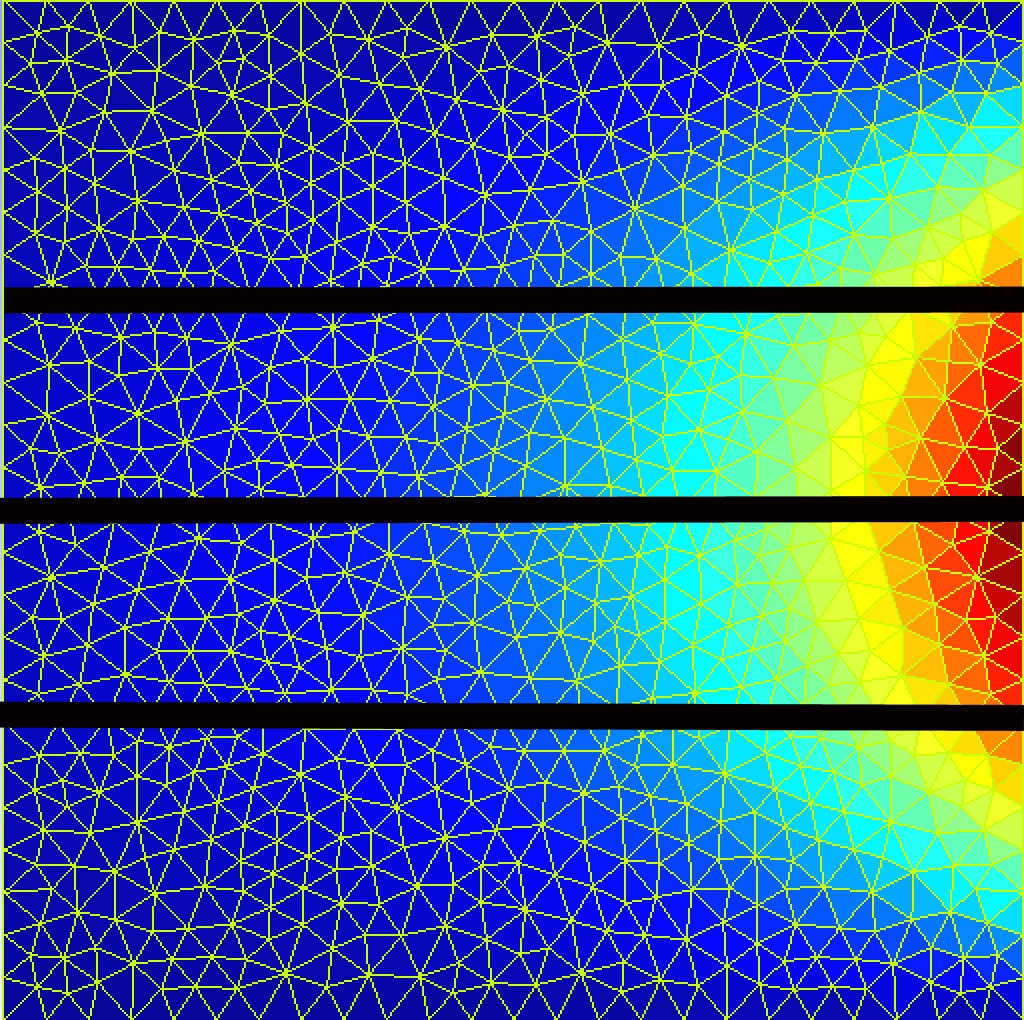
\includegraphics[width=.6\textwidth]{../images/meshhorizontal.png}        
	\end{figure}
\end{frame}

\begin{frame}
	\begin{figure}[!htp]
    	\centering   
        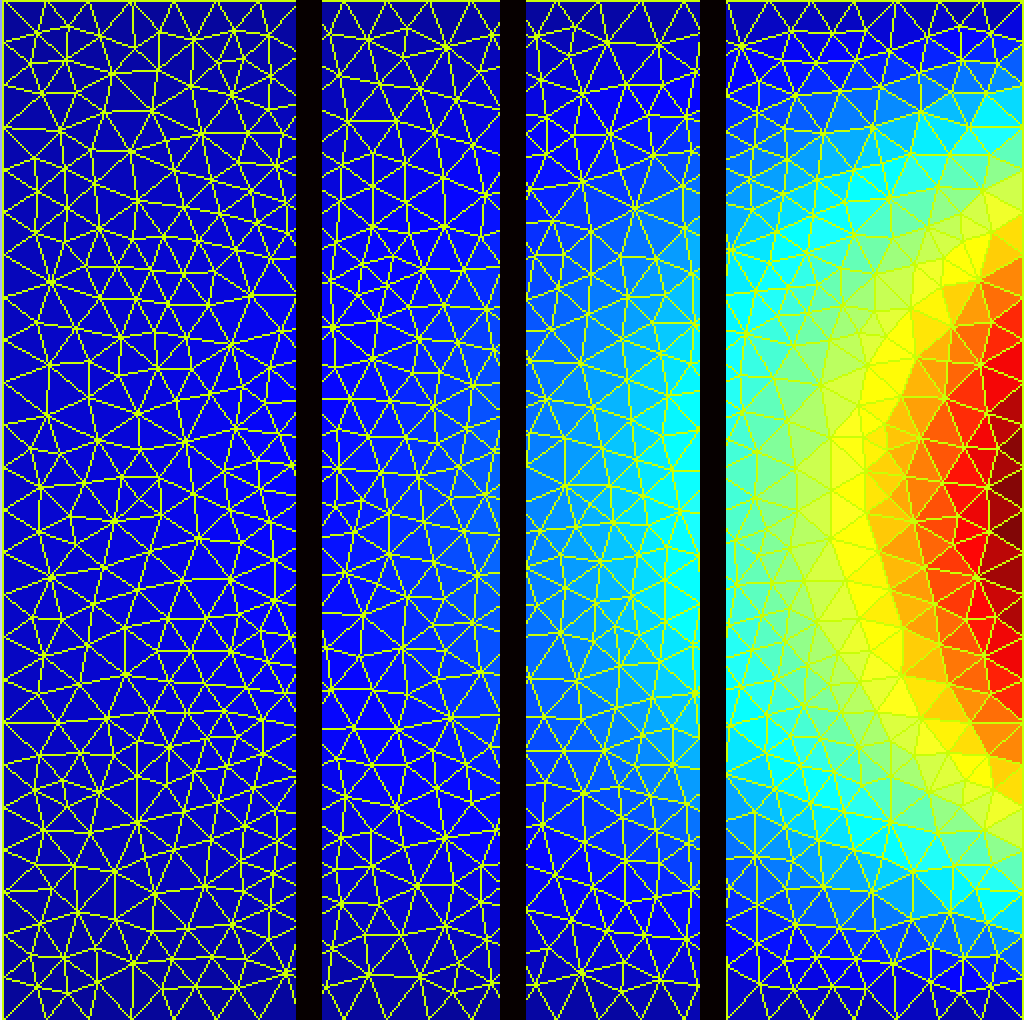
\includegraphics[width=.6\textwidth]{../images/mesh_vertical.png}        
	\end{figure}
\end{frame}




\subsection{Final Implementation}

\begin{frame}
	\frametitle{Optimizations}
	\begin{columns}
		\smaller
		\column{0.4\textwidth}
			\centering
			\textbf{\itshape Array-Of-Structs}

			\smaller
			\begin{tabular}{|c|c|}
				\hline
				\multirow{4}{*}{$S_{1}$} & $e_{1}$\\
				\cline{2-2}
				& $e_{2}$\\
				\cline{2-2}
				& $e_{3}$\\
				\cline{2-2}
				& \ldots\\
				\hline
				\multirow{4}{*}{$S_{2}$} & $e_{1}$\\
				\cline{2-2}
				& $e_{2}$\\
				\cline{2-2}
				& $e_{3}$\\
				\cline{2-2}
				& \ldots\\

				\hline
				\multirow{5}{*}{$S_{3}$} & $e_{1}$\\
				\cline{2-2}
				& $e_{2}$\\
				\cline{2-2}
				& $e_{3}$\\
				\cline{2-2}
				& \dots\\
				\hline
				\multicolumn{2}{|c|}{\ldots}
			\end{tabular}
			\larger

			\begin{itemize}
				\item Pointers $\Rightarrow$ Indexes;
			\end{itemize}

		\column{0.4\textwidth}
			
			\centering
			\textbf{\itshape Structs-Of-Arrays}

			\smaller
			\begin{table}
				\captionsetup[subfloat]{position=top,labelformat=empty}
				\subfloat[$e_{1}$]{%
				\begin{tabular}{|c|}
					\hline
					$S_{1}$\\
					\hline
					$S_{2}$\\
					\hline
					$S_{3}$\\
					\hline
					\ldots
				\end{tabular}%
				}\;
				\subfloat[$e_{2}$]{%
				\begin{tabular}{|c|}
					\hline
					$S_{1}$\\
					\hline
					$S_{2}$\\
					\hline
					$S_{3}$\\
					\hline
					\ldots
				\end{tabular}%
				}\;
				\subfloat[$e_{3}$]{%
				\begin{tabular}{|c|}
					\hline
					$S_{1}$\\
					\hline
					$S_{2}$\\
					\hline
					$S_{3}$\\
					\hline
					\ldots
				\end{tabular}%
				}\;
				\subfloat[\ldots]{}
			\end{table}
			\larger

			\begin{itemize}
				\item Pointers $\Rightarrow$ Indexes;
				\item Loads only what is needed;
			\end{itemize}
	\end{columns}
\end{frame}

\begin{frame}
\titlepage
	\begin{center}
		\Huge\bfseries
		- ? -
	\end{center}
\end{frame}

\end{document}%	end presentation